Computational biology involves the development and application of data-analytical and theoretical methods, mathematical modelling and computational simulation techniques to the study of biological, behavioural, and social systems. The field is broadly defined and includes foundations in computer science, applied mathematics, animation, statistics, biochemistry, chemistry, biophysics, molecular biology, genetics, genomics, ecology, evolution, anatomy, neuroscience, and visualization.
Computational biology is different from biological computation, which is a subfield of computer science and computer engineering using bioengineering and biology to build computers, but is similar to bioinformatics, which is an interdisciplinary science using computers to store and process biological data.
Computational Biology, which includes many aspects of bioinformatics, is the science of using biological data to develop algorithms or models to understand among various biological systems and relationships. Until recently, biologists did not have access to very large amounts of data which have become commonplace, particularly in molecular biology and genomics. Researchers were able to develop analytical methods for interpreting biological information, but were unable to share them quickly among colleagues.
\section{Bioinformatics}
Bioinformatics is the use of computers for the acquisition, management, and analysis of biological information.
It incorporates elements of molecular biology, computational biology, database computing, and the Internet. Bioinformatics is clearly a multi-disciplinary field including: computer systems management networking, database design, computer programming, and molecular biology.
Bioinformatics is both an umbrella term for the body of biological studies that use computer programming as part of their methodology, as well as a reference to specific analysis "pipelines" that are repeatedly used, particularly in the field of genomics. Common uses of bioinformatics include the identification of candidate genes and single nucleotide polymorphisms (SNPs). Often, such identification is made with the aim of better understanding the genetic basis of disease, unique adaptations, desirable properties (esp. in agricultural species), or differences between populations. In a less formal way, bioinformatics also tries to understand the organisational principles within nucleic acid and protein sequences, called proteomics.

\begin{figure}[ht]
\centering
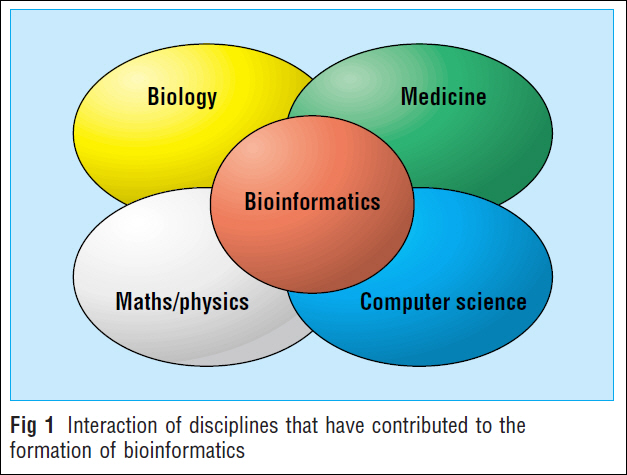
\includegraphics[scale=0.5]{images/bio.png}
\caption{Bioinformatics}
\end{figure}


\section{Sequence Analysis}
\begin{enumerate}
\item DNA SEQUENCING


Before sequences can be analyzed they have to be obtained. DNA sequencing is still a non-trivial problem as the raw data may be noisy or afflicted by weak signals. Algorithms have been developed for base calling for the various experimental approaches to DNA sequencing.
\item SEQUENCE ASSEMBLY


Most DNA sequencing techniques produce short fragments of sequence that need to be assembled to obtain complete gene or genome sequences. The so-called shotgun sequencing technique generates the sequences of many thousands of small DNA fragments
\item GENOME ANNOTATION


In the context of genomics, annotation is the process of marking the genes and other biological features in a DNA sequence. This process needs to be automated because most genomes are too large to annotate by hand, not to mention the desire to annotate as many genomes as possible, as the rate of sequencing has ceased to pose a bottleneck.
\end{enumerate}
